\chapter{Methods}
\label{chap:meth}
\lettrine[lines=4, loversize=-0.1, lraise=0.1]{T}{he following chapter} will present the research questions that were the core of the thesis as well as the methods and experiments used during this research. The chapter will describe how the experiments were performed and their motivation and purpose.
\section{Design Research}
%Because an integration between speech-recognition software and requirement annotations never had been done before, a design research was carried out. The design research had the main focus on developing a product for annotating SRSs with speech recognition. Alongside with the development of the product, different methods where conducted to evaluate and investigate what the product could contribute with. 
The main objectives of the thesis was to answer the research questions seen below. To be able to answer these, a design research was carried out by the development of SpeechWeaver (see Chapter \ref{cha:techsol}). 

\begin{framed}
\begin{flushleft}
    \textbf{RQ1:} How do you connect the annotation-data to a requirement?
    
    \textbf{RQ2:} How do you adapt annotations for working with mobile speech recognition?
    
    \textbf{RQ3:} How does the user experience the interaction with mobile speech recognition
    software in the context of Software Requirement Specifications.
    
    \textbf{RQ4:} How can you aggregate the annotations in a presentable and usable way?
    
    \textbf{RQ5:} Is speech recognition annotations scalable on large Software Requirement Specifications
\end{flushleft}
\end{framed}

The design research was preceded by interviews to elicit requirements on SpeechWeaver, as well as gaining knowledge about SystemWeaver, the subjects background and how they worked with requirement management and SystemWeaver. The design research was complemented with four evaluation steps as shown in Figure~\ref{fig:resov}.
Steps 1 and 2 focused on evaluating to what degree output from speech recognition is useful for identification (step 1) and free-text annotation (step 2) of requirements.
Scaling to realistic requirements database sizes is critical for industrial applicability and since the response time of the system was considered a key characteristic by the company and the identification of requirements dominated the round-trip time, evaluation step 3 measured this time on the server for four different requirement sets.
Finally, step 4 evaluated the SpeechWeaver through a user test and a follow-up interview.
Below we describe the evaluation steps in detail.



%In Figure~\ref{fig:methodoverview}, an overview of the thesis is visualized. The thesis was based on the five research questions. The purpose of the methods chosen for the thesis (\textbf{M0-M5}} was to give clarity to those questions.

%\begin{figure}[h]
%\centering
%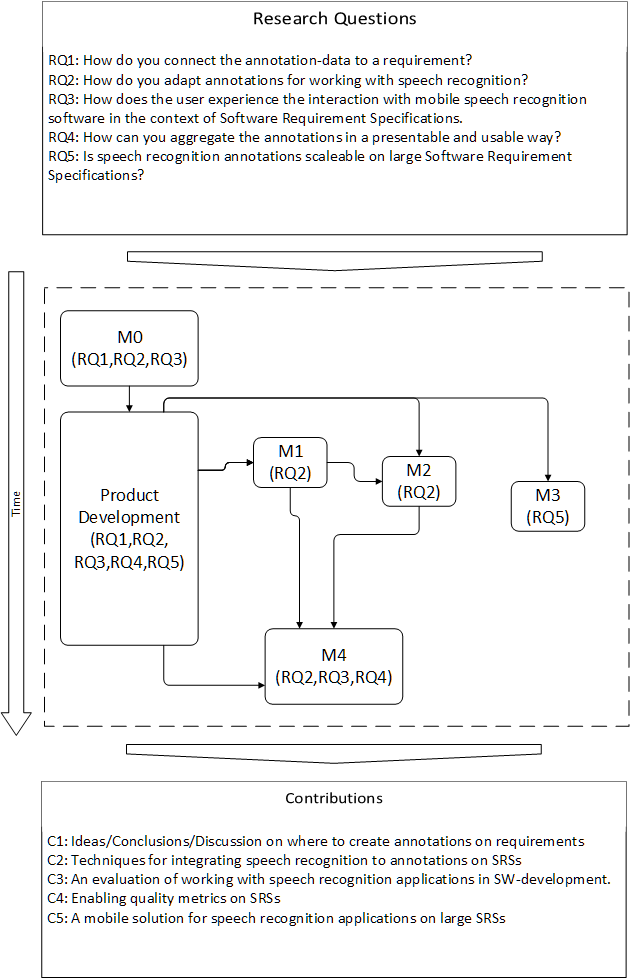
\includegraphics[width = 340pt, keepaspectratio = true]{fig/MethodSummary.png}
%\caption{The structure of the thesis. The product development (see section~\ref{subsec:devel}) contained the implementation of the product. \textbf{RQ\#} Research questions. \textbf{C\#} Conclusions.} \textbf{M\#} Methods conducted during the thesis.
%\label{fig:methodoverview}
%\end{figure}
%\FloatBarrier

\begin{figure}[h]
\centering
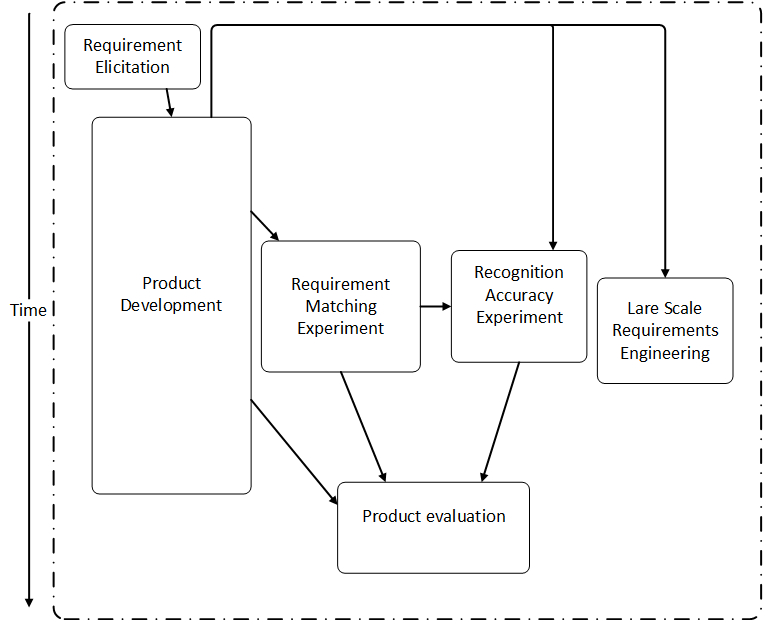
\includegraphics[width = 400pt, keepaspectratio = true]{fig/methodsummarythesis.png}
\caption{An overview of the design research.}
\label{fig:resov}
\end{figure}
\FloatBarrier
%The thesis contained an elicitation interview (\textbf{M0}, see section~\ref{subsec:elicitationint}), two experiments to evaluate state of practice speech recognition (\textbf{M1}, see section~\ref{sec:reqmatchexp}, \textbf{M2}, see section~\ref{sec:speechrecacc}), an evaluation of the scalability for large scale requirement engineering (\textbf{M3}, see section~\ref{sec:largere}) and a product evaluation containing a user test and a follow-up interview (\textbf{M4}, see section~\ref{sec:usertestusa}). 

\subsection{Development}
\label{subsec:devel}
The product was developed with an agile process. The main objectives of the product was:

\begin{itemize}
  \item \textbf{The main action for giving the system input should be through speech: }To be able to investigate and evaluate how well a speech recognizer behaves in a technical domain.
  \item \textbf{To create a connection between the mobile smart device application and a requirement database: } To be able to utilize the mobility offered by a smartphone to annotate SRSs.
  \item \textbf{Annotations on requirements: }To investigate how a requirement could be annotated from a technical perspective (e.g.\ as meta-data or as an attribute etc)
  \item \textbf{Extract the annotation data from the requirements: }To visualize and analyze the data that the annotations provided.
\end{itemize}

The sprint lengths for the project was one week. The smart device application and SpeechServer as described in chapter~\ref{cha:techsol} were developed in parallel. The solutions aimed to be as general as possible to prove the concept of annotating requirement entities.

\subsection{Requirement Elicitation}
\label{sec:elicitation}
The requirements on the system originated from the the authors as product owners, as well as from interviews and discussions with requirement engineers, application engineers and software developers at Systemite AB. After each sprint new problems were identified, requirements were elicited and prioritized, which allowed for an adaptive and responsive process. 

\subsubsection{Interview}
\label{subsec:elicitationint}
In the very beginning of the thesis an interview was conducted to give an understanding about the background information of SystemWeaver and requirement management today, but also to elicit requirements on the system that was developed. The interview subjects were application engineers and software developers at Systemite with a span of three to ten years of experience in requirement management. The elicitation interview focused on four main objectives. \\

\begin{itemize}
    \item \textbf{Personal information:} To get an understanding of the subjects educational background and experiences, as well as their role in the company and their usage of SystemWeaver.
    \item \textbf{SystemWeaver:} Since the smart device would be integrated with SystemWeaver, the purpose was to get a better understanding of SystemWeaver's semantics, structure, flaws and advantages. It was also necessary to find out how companies and people use SystemWeaver.
    \item \textbf{Requirement management:} To get insight into how people who work with requirement and SRSs every day experiences how the change management and maintenance of the documents functions.
    \item \textbf{Speech recognition:} A brief questioning about if the subject had any earlier experience with speech recognition software, and if so, what advantages and limitations they felt the software had.
\end{itemize}

The questions that the interviews were based on can be found in appendix \ref{app:intquest}

\section{Requirement Matching Experiment}
\label{sec:reqmatchexp}
Even though speech recognition algorithms have improved in recent years the error rates can still be high.
This is especially true for the speech recognition available in mobile devices which is typically speaker-independent (which has higher error rates) and has a limited compute power.
Our initial results also confirmed that there was often a large discrepancies between the intended requirements supplied as speech input and the output from the speech recognizer.
To make requirements identification possible we extended the system with the Levenshtein string distance as described in sectino~\ref{subsubsec:stringmetric}.
%When using speech recognizers, there is room for the speech recognition engine to make interpretational errors. A core function in our product was to make up for those errors, something that was done using a string edit distance function when the speech recognizer did not catch the exact sentence that were given through speech. 
To evaluate how well this solution performed an experiment was conducted.

The experiment had 10 subjects, all who were students at Chalmers University of Technology, and all with English as their second language. 
Each student was given 10 randomly selected requirement titles from an SRS with 4544 requirements and were asked to speak the titles into the speech recognizer. 
The most likely output from the speech recognizer was then saved and used to evaluate lookup of requirements in that SRS through the Levenshtein edit-distance algorithm.
%The length of the interpreted input and the length of the target requirement title, and the difference between those, were saved for analyzing.
For each input we noted the input length (string length of output from speech recognizer), the target requirement length, distances from input to all requirement titles in the SRS, as well as the rank of the target requirement in the ranking created by the distance function.
An example of the data saved for each input can be found in Table \ref{tab:experimentexample} 

The algorithm was extended to also check for perfect matches (i.e. the interpreted input was exactly the same as the requirement title), and if it was found, the position of the returned result from the speech recognizer were saved. This extension was made to utilize that the speech recognizer returned five different interpretations of the spoken input. If a perfect match was found in any of the five results, the input was never run through the distance function. If a perfect match was not found, only the most likely result from the speech recognizer was run through the distance function. 

\begin{framed}
    \begin{center}
    {\LARGE \sc Requirement matching experiment design}
    \begin{description}
    \item [Purpose:] To evaluate how a string edit distance function can help to find a sought requirement in a specific SRS.
    \item [Motivation:] Because there are inaccuracies in speech recognizers, we want to investigate and evaluate how string edit distance function can help mitigate the accuracy problems by returning similar strings to the given input.
    \item [Subject Sample:] 10 randomly selected students from the Software Engineering programme at Chalmers University of Technology (both undergraduate students and graduate students). The subject have English as their second language.
    \item[Experiment Setup:] The requirement titles (which is a short description of the requirement, the human readable ID) are taken from an SRS from automotive industry , and the context within that SRS which has the most requirements in it (a context is defined as a delimited part of an SRS such as different abstraction levels (e.g.\ Analysis Level, Design Level, Implementation Level)). 10 requirements for each subject are randomly taken from the the selected context. 
    \item[Execution:] The subject is asked to say each of the 10 selected requirements. The requirement titles are shown to the subjects on a screen. Each input of a title is followed by a pause and the subject will have as much time as they need to read and prepare for the next input.

    For each requirement title, the input is recorded by an Android device and the results from the speech recognition engine (see section~\ref{sec:sr}) are recorded in a file. Each subject's data will be recorded in separate files.
    \item[Evaluation:] From the files, the best result for each requirement title is run through the requirement matching algorithm to find what ranking it places the correct requirement. The ranking is based on the requirement title's string edit distance in comparison with all other requirement titles' string edit distances in the same context (using Levenshtein edit distance algorithm, an example is illustrated in Table~\ref{tab:experimentexample}).
    The evaluation will also look at \emph{perfect matches}, which is defined as 1 of the 5 results from the speech engine being exactly the same as the sought requirement title (it will also look at how often these occur and how often a perfect match is found, but it is not the correct requirement).
    \end{description} 
    \end{center}
\end{framed}

\begin{table}[h]
    \centering
    \caption{Table showing how Levenshtein distance and ranking is calculated for a given input in a closed domain of requirement titles.}
        \begin{tabular}{ l l l l }
            \hline
            Input & Requirement titles & Distance & Rank\\
            \hline
            And its allies buffet & Initialize buffer & 9 & 1 \\
    %        \hline
             & Erroneous APLM buffer & 15 & 3 \\
   %          \hline
             & State monitoring buffer & 14 & 2 \\
  %           \hline
             & Transaction: Buffer on - Buffer off & 26 & 5 \\ 
    %         \hline
             & Buffer out of range & 18 & 4 \\ 
   %          \hline
            \end{tabular}
    \label{tab:experimentexample}
\end{table}


\section{Recognition Accuracy Experiment}
Experiment 2 was conducted to evaluate how the speech recognizer behaved with free text input.
Even if this is a typical use of speech recognition we are targeting a specific, technical domain and not everyday speech/text.
Thus, the performance of speech recognition can be expected to be worse.
Since free-form speech recognition would be needed in allowing arbitrary annotations to requirements this is a key concern for our application.

%from a technical domain in a technical domain. 
From the same SRS as mentioned above (see section \ref{sec:reqmatchexp}), 100 sentences were randomly selected . 
The same 10 students as mentioned above were then asked to speak 10 of the sentences into the speech recognizer.
%rf: If it is the same 10 students and 100 requirements it's better to say that.

%O&V säger nu att det vara samma som tidigare nämnts
The best interpreted result from the speech recognizer was then saved in a text file and were later given a value between 0-3, were the numeric defined the level of severeness of the error, as can be seen in Table \ref{tab:severity}. The design of the experiment can be seen below.


\label{sec:speechrecacc}
\begin{framed}
    \begin{center}
    {\LARGE \sc Recognition Accuracy Experiment Design}
    \begin{description}
    \item [Purpose:] To find out how accurate speech to text as input is for technical descriptions of requirements.
    \item [Motivation:]
    To investigate the speech recognizers accuracy on sentences and evaluate if it is a viable option to have as free text input towards technical domains.
    \item [Subject Sample:] 10 randomly selected students from the Software Engineering programme at Chalmers University of Technology (both undergraduate students and graduate students). The subject have English as their second language. (Same subjects as in the Requirement matching experiment)
    \item [Experiment Setup:] 100 sentences are taken from the description from the same requirements as in Requirement Matching Experiment~\ref{sec:reqmatchexp} 
    \item [Execution:] The subject each says ten of the sentences. The input is recorded by the Android speech recognizer, and the interpreted inputs are saved in a file.
    \item [Evaluation:] The evaluation will look at the \emph{severity} of the input error on a scale of 0-3 as described in Table~\ref{tab:severity}. The result is presented in a table to see how much errors are introduced by the free text speech input.
    
    \end{description}
    \end{center}
\end{framed}

\begin{table}[h!]
    \centering
    \caption{Table showing interpretations of severity.}
        \begin{tabular}{ l p{8cm} }
            \hline
            Severity & Meaning \\
            \hline
            0 & No error \\
            1 & Minor error, still comprehensible \\
            2 & Error, hard/impossible to comprehend \\
            3 & Severe Error, meaning of text has changed, but has a viable meaning in the context \\
            \end{tabular}
    \label{tab:severity}
\end{table}

\section{Large Scale Requirements Engineering}
\label{sec:largere}
Software projects out in the industry can be very large in terms of complexity and size. To evaluate how scalable our solution was, a test suite was ran on medium-scaled and large-scaled SRSs \citep{regnell2008} taken from the automotive industry.

The purpose was to test how the product behaved on different sized software projects, and variables were measured when the product was in action. The variables that were interesting to look at were:


\begin{description}
\item [SRS size:] The number of requirements within the SRS
\item [Execution time:] How much time (in milliseconds) it took from the moment the server received the input until it have fetched the results, and is ready to send to the client. This to evaluate how the system scales in execution time.

\end{description}
For each of the SRSs, a requirement was identified. A user then gave the name of the identified requirement as input to the system through speech. Each SRS was queried 30 times and the different values for the above mentioned variables where then saved for analysis.

\section{Product Evaluation}
\label{sec:usertestusa}
The end user evaluation of SpeechWeaver contained two parts, monitored user tests followed by interviews. 
The subjects for the user test was five requirement- and application-engineers at Systemite AB.

The subjects was given a short introduction about the features and the design of the application and was then given five randomly selected requirements within a chosen context and was asked to create an issue to each of the requirement with the application. Out of these five, two of the issues required an attached file (see Section \ref{subsec:usage}). After the requirements were annotated the user sat down and explored the result of the actions by looking at the updates that had been added in SystemWeaver (see Section ~\ref{sec:SystemWeaver}). Finally the user was interviewed about the experience of using the application. The main focus of the interview was the experience of using speech as input, but also overall impressions of the usability and ease of use of the product as a whole. The questions the interview was based on can be seen in Appendix \ref{app:evalint}.













